\documentclass{standalone}

\usepackage{pgfplots}
\usepackage{amsmath, amssymb}
\usepgfplotslibrary{fillbetween}
\pgfplotsset{compat=1.18}

\begin{document}

%==================================================
% Forward Euler
%==================================================
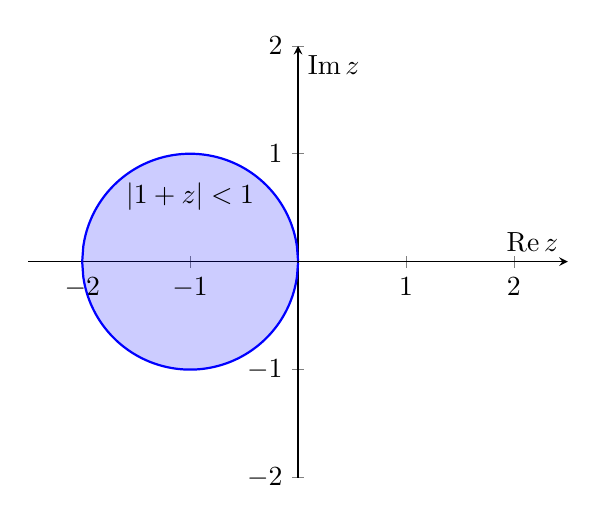
\begin{tikzpicture}[baseline]
    \begin{axis}[
        % width=8cm,
        % height=7cm,
        axis lines=middle,
        xlabel={$\operatorname{Re} z$},
        ylabel={$\operatorname{Im} z$},
        xmin=-2.5, xmax=2.5,
        ymin=-2, ymax=2,
        axis equal image,
        samples=200,
        domain=-2:0,
    ]
        % Upper half of |1+z|=1
        \addplot[name path=FEupper, draw=blue, thick]{sqrt(1-(x+1)^2)};
        % Lower half
        \addplot[name path=FElower, draw=blue, thick]{-sqrt(1-(x+1)^2)};
        % Absolute stability region
        \addplot[blue, opacity=0.2] fill between[of=FEupper and FElower];
        \node at (axis cs:-1,0.6) {$|1+z|< 1$};
    \end{axis}
\end{tikzpicture}

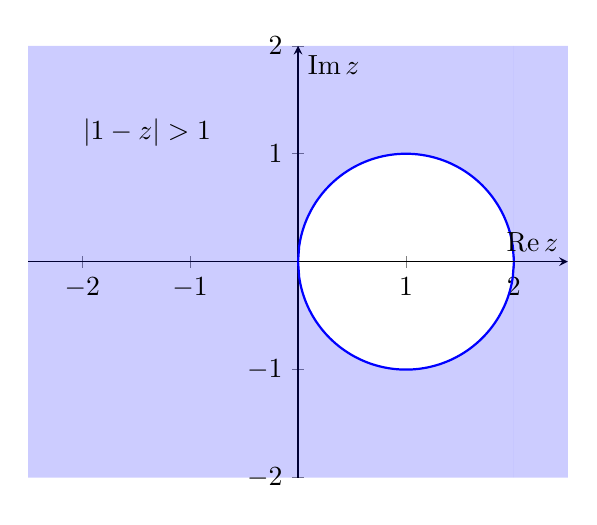
\begin{tikzpicture}[baseline]
    \begin{axis}[
        % width=8cm,
        % height=7cm,
        axis lines=middle,
        xlabel={$\operatorname{Re} z$},
        ylabel={$\operatorname{Im} z$},
        xmin=-2.5, xmax=2.5,
        ymin=-2, ymax=2,
        axis equal image,
        samples=200,
    ]
        % Plot boundary separately
        \addplot[blue, thick, domain=0:2]{sqrt(1-(x-1)^2)};
        \addplot[blue, thick, domain=0:2]{-sqrt(1-(x-1)^2)};
        % Upper boundary of plotting box
        \addplot[name path=top, draw=none, domain=-3:3]{2};
        % Upper part of circle
        \addplot[name path=BEupper, draw=none, domain=0:2]{sqrt(1-(x-1)^2)};
        % Lower part of circle
        \addplot[name path=BElower, draw=none, domain=0:2]{-sqrt(1-(x-1)^2)};
        % Lower boundary of plotting box
        \addplot[name path=bottom, draw=none, domain=-3:3]{-2};
        % Left region: automatically stable
        \path[name path=leftline] (axis cs:0,-2) -- (axis cs:0,2);
        \addplot[blue, opacity=0.2] fill between [of=top and bottom, soft clip={domain=-3:0}];
        % Region above the circle
        \addplot[blue, opacity=0.2] fill between [of=top and BEupper, soft clip={domain=0:2}];
        % Region below the circle
        \addplot[blue, opacity=0.2] fill between [of=BElower and bottom, soft clip={domain=0:2}];
        % Right of the circle
        \addplot[blue, opacity=0.2] fill between [of=top and bottom, soft clip={domain=2:3}];
        \node at (axis cs:-1.4,1.2) {$|1-z|> 1$};
    \end{axis}
\end{tikzpicture}

\end{document}